
\newcommand{\toyfigwidth}{0.9\textwidth}
\begin{figure}[!htbp]
    \centering
    \begin{tabular}{@{}c@{}}
        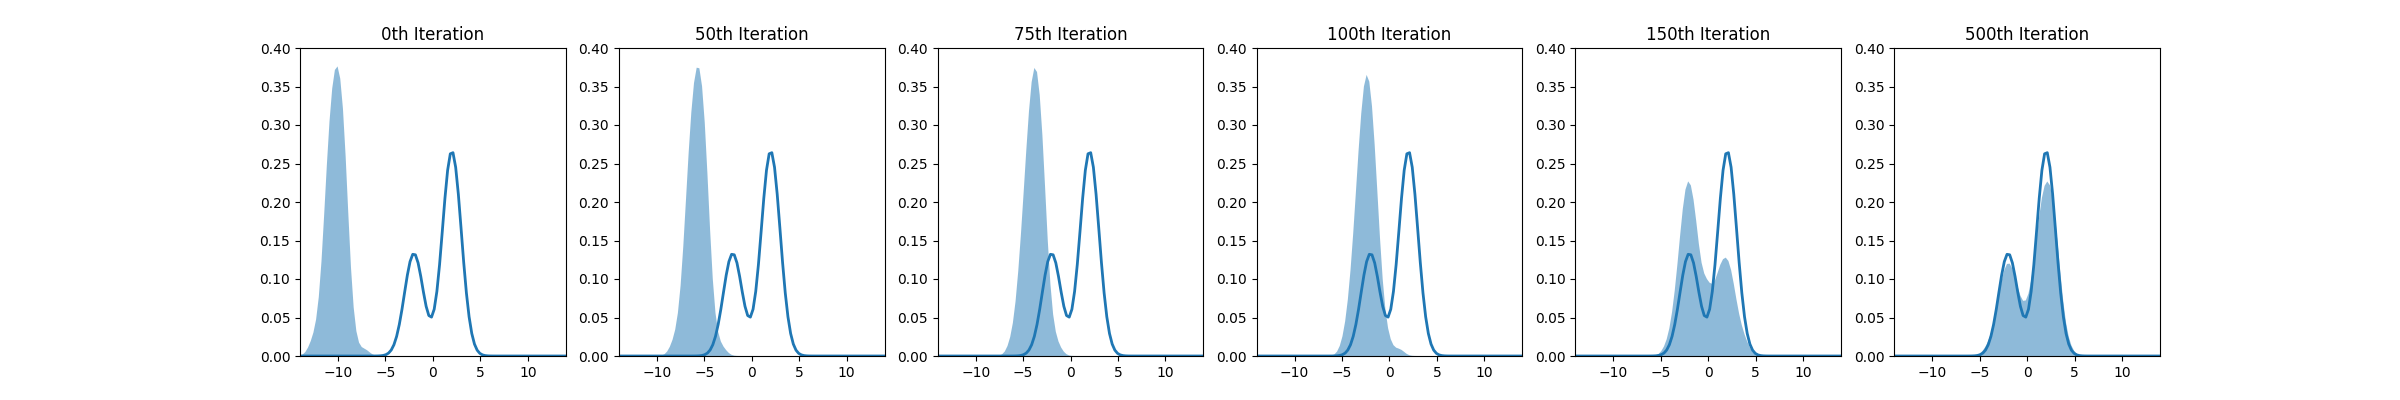
\includegraphics[width=\toyfigwidth]{figs/toy-figure1_step0.1_mu2.0_w0.33_gaussian.png} \\
        \small (1) StepSize = 0.1, 500 iterations, $\mu = \pm 2$, $(w_1, w_2) = (0.33, 0.67)$
    \end{tabular}
    
    \begin{tabular}{@{}c@{}}
        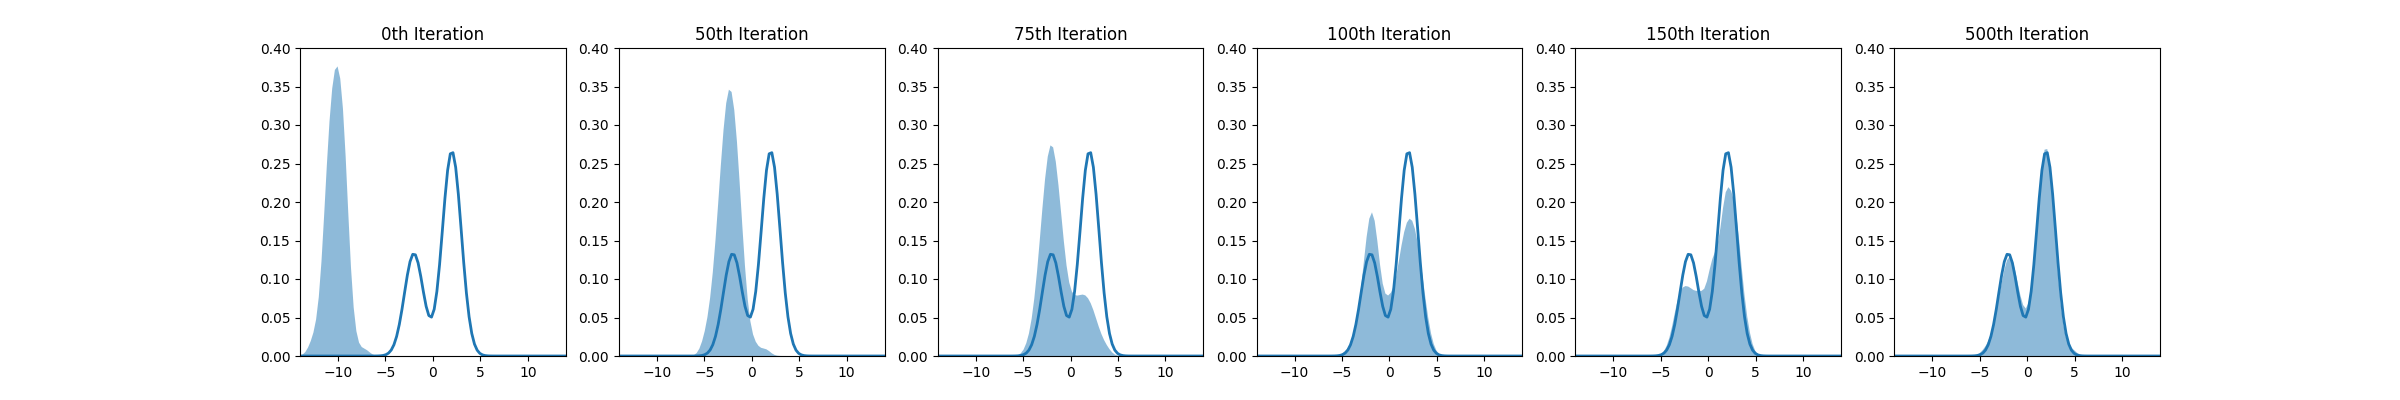
\includegraphics[width=\toyfigwidth]{figs/toy-figure1.png} \\
        \small (2) StepSize = 0.25, 500 iterations, $\mu = \pm 2$, $(w_1, w_2) = (0.33, 0.67)$
    \end{tabular}
    %\vspace{\floatsep}
    
    \begin{tabular}{@{}c@{}}
        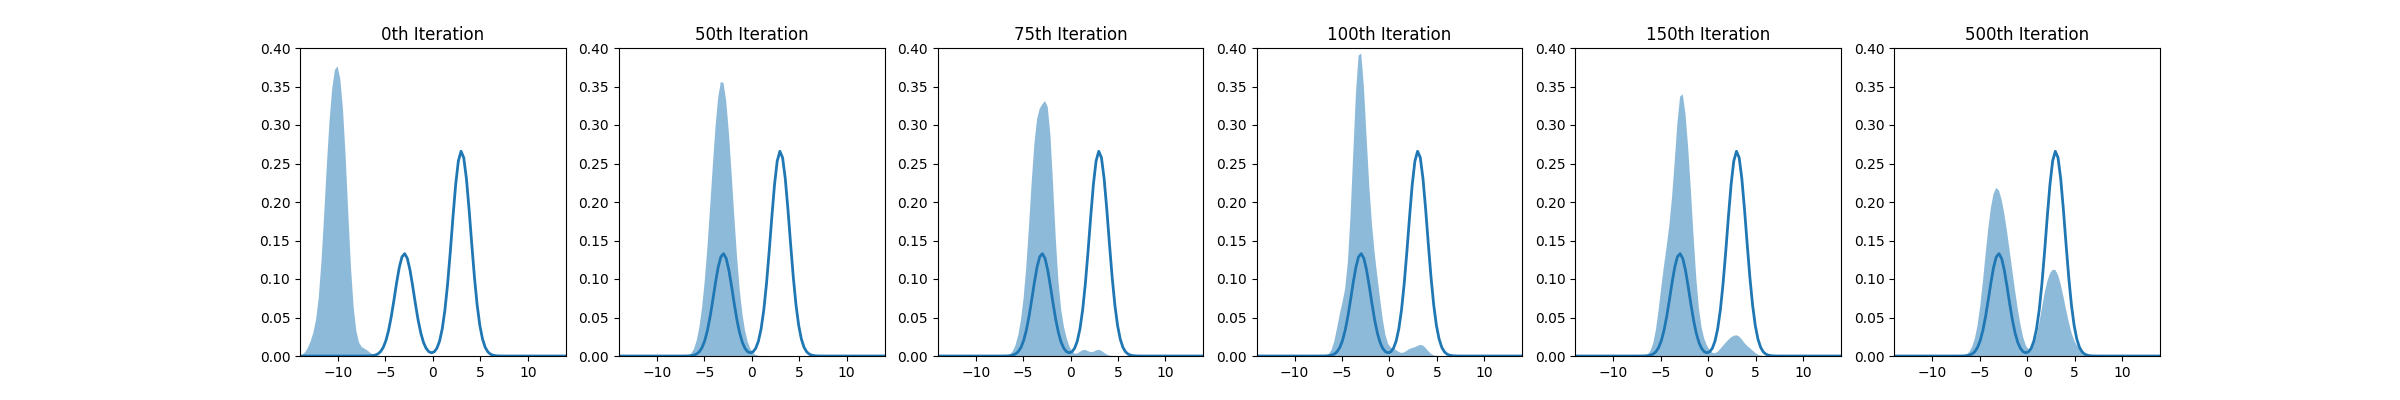
\includegraphics[width=\toyfigwidth]{figs/toy-figure1_step0.25_mu3.0_w0.33_gaussian.png} \\
        \small (3) StepSize = 0.25, 500 iterations, $\mu = \pm 3$, $(w_1, w_2) = (0.33, 0.67)$
    \end{tabular}
    
    \begin{tabular}{@{}c@{}}
        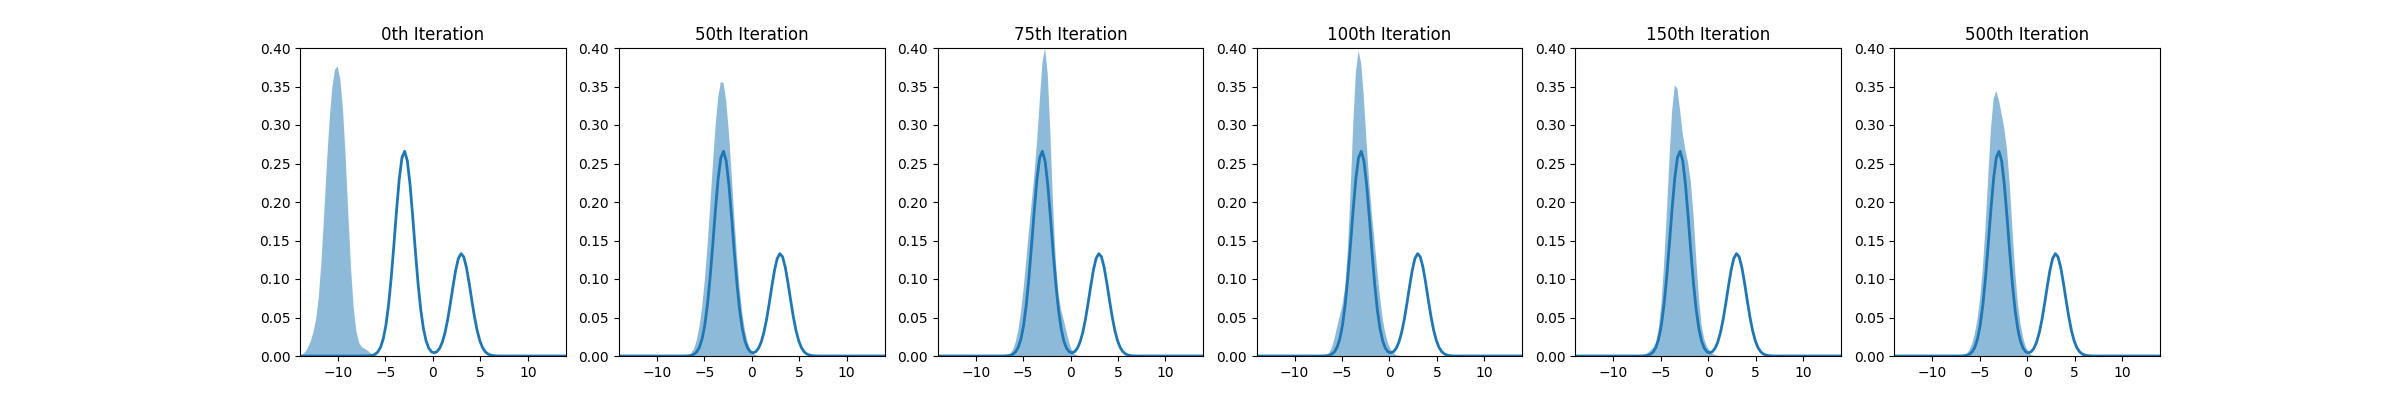
\includegraphics[width=\toyfigwidth]{figs/toy-figure1_step0.25_mu3.0_w0.67_gaussian.png} \\
        \small (4) StepSize = 0.25, 500 iterations, $\mu = \pm 3$, $(w_1, w_2) = (0.67, 0.33)$
    \end{tabular}
    
    % \begin{tabular}{@{}c@{}}
    %     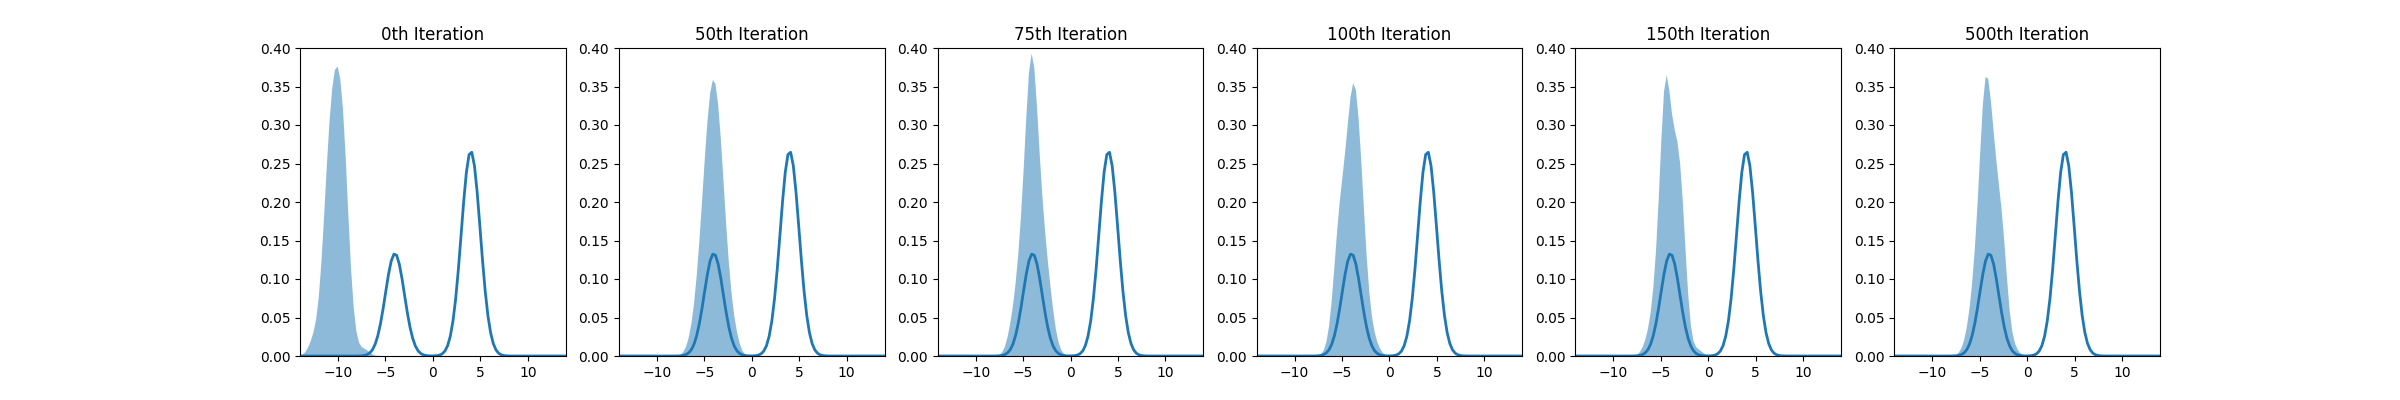
\includegraphics[width=\textwidth]{figs/toy-figure1_step0.25_mu4.0_w0.33_gaussian.png} \\
    %     \small (5) StepSize = 0.25, $\mu = \pm 4$, $(w_1, w_2) = (0.33, 0.67)$
    % \end{tabular}
    
    \begin{tabular}{@{}c@{}}
        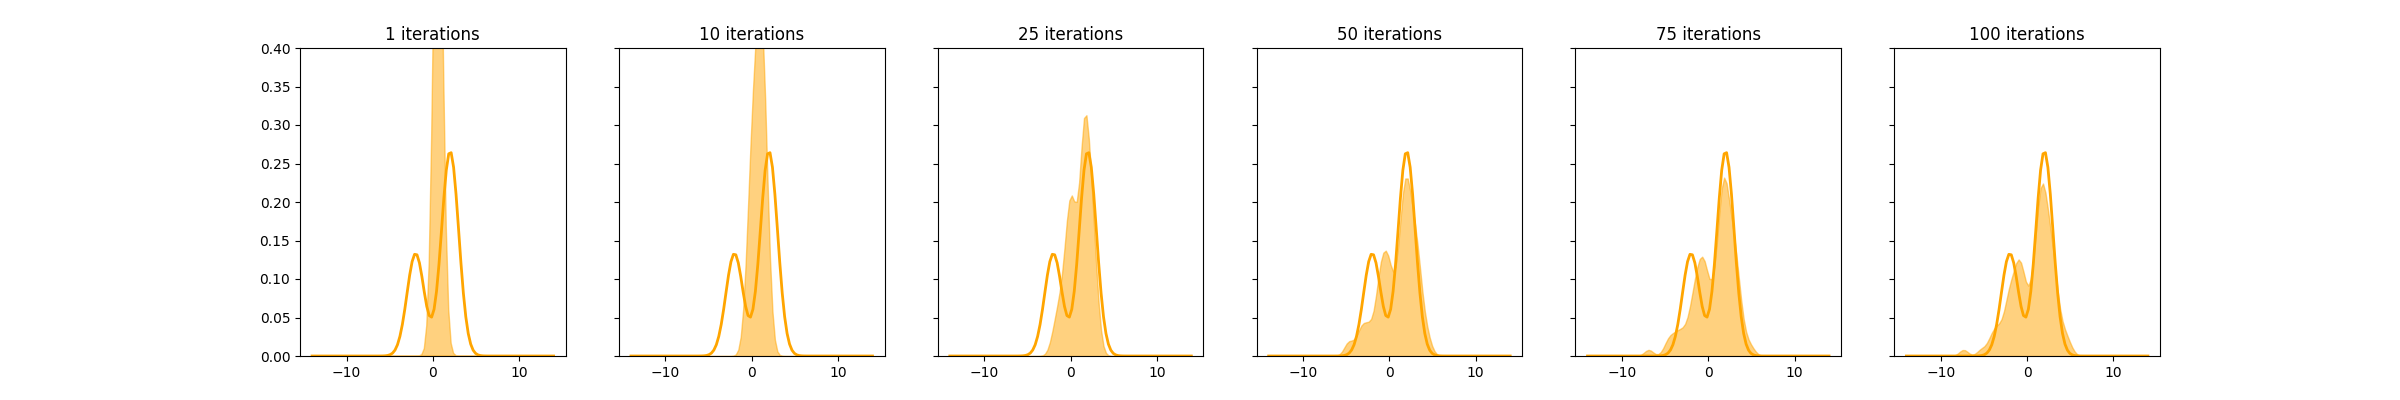
\includegraphics[width=\toyfigwidth]{figs/toy-figure1-numpyro.png} \\
        \small (5) ELBO Loss (NumPyro) StepSize = 0.1, 100 iters, $\mu = \pm 3$, $(w_1, w_2) = (0.33, 0.67)$
    \end{tabular}
     
    \caption{Toy example with 1D Gaussian mixture. Particle densities are visualized by KDE.}
    \label{fig:toy1dgaussian}
\end{figure}
